 \section{Sensores}
	Los sensores son dispositivos que permiten a los robots percibir su entorno y obtener información sobre su posición, movimiento, temperatura, proximidad, presión, entre otros aspectos. Estos sensores convierten datos físicos en señales eléctricas que el robot puede procesar para tomar decisiones o realizar tareas.

Se clasifican en:

	\subsection{Sensores Internos}
		\begin{enumerate}
			\item \textbf{Posición}
			\begin{enumerate}
				\item Lineal y rotativo
				\begin{enumerate}
					\item Encóder incremental
					\item Potenciómetro
					\item LVDT
					\item Resólver
				\end{enumerate}
			\end{enumerate}
			
			\item \textbf{Velocidad}
			
            Los sensores de velocidad realizan la medición tomando medidas de posición consecutivas a intervalos de tiempo constante, calculando la razón de cambio respecto al tiempo de los valores de posición, o lo determina en forma directa con base en diferentes principios.\cite{saha2010robotics}\\
           
			
			\begin{enumerate}
				\item Todos los sensores de posición:
				Básicamente todos los sensores de posición, cuando se utilizan con ciertos límites de tiempo, pueden dar la velocidad, por ejemplo, el número de pulsos proporcionados por un encóder de posición incremental dividido entre el tiempo consumido en hacerlo. Sin embargo, este método impone una carga computacional sobre el controlador, que podrá estar ocupado por algunas otras operaciones.\\
		
		\begin{figure}[!ht]
			\centering
			\subfloat[Sensores de posición]{%
				\includegraphics[width=0.3\textwidth]{Velocidadsensoresdeposición.jpg}%
				\label{fig:sensores}
				\cite{Sensordeposición}
			}
			\hfill
		\end{figure}
				
				\item Tacómetro: Estos sensores pueden encontrar directamente la velocidad en cualquier momento y sin mucha carga computacional. Éstos miden la velocidad de rotación de un elemento. Hay varios tipos de tacómetros en uso, pero un diseño sencillo se basa en la regla de Fleming, que declara que “el voltaje producido es proporcional al índice del acoplamiento inductivo”. Aquí un conductor (básicamente una bobina) se sujeta al elemento rotativo que gira en un campo magnético (estator). Conforme incrementa la velocidad del eje, el voltaje producido en las terminales de las bobinas también aumenta.\cite{saha2010robotics}\\
				
				\begin{figure}[h]
					\centering
					\subfloat[Tacómetro]{%
						\includegraphics[width=0.3\textwidth]{Tacómetro.jpg}%
						\label{fig:Tacómetro}
						\cite{Tacómetro}
					}
					\hfill
				\end{figure}
				
				\item Sensor de efecto Hall: Es un dispositivo que se utiliza para medir la magnitud de un campo magnético. Su función se basa en el fenómeno físico conocido como el efecto Hall, por el cual se genera una diferencia de potencial eléctrico, o voltaje Hall, a través de un material conductor cuando este se encuentra dentro de un campo magnético y se le hace pasar una corriente eléctrica. Este fenómeno fue descubierto en 1879 por el físico estadounidense Edwin Hall.\cite{Hall} \\
				
			\begin{figure}[h]
				\centering
				\subfloat[EfectoHall]{%
					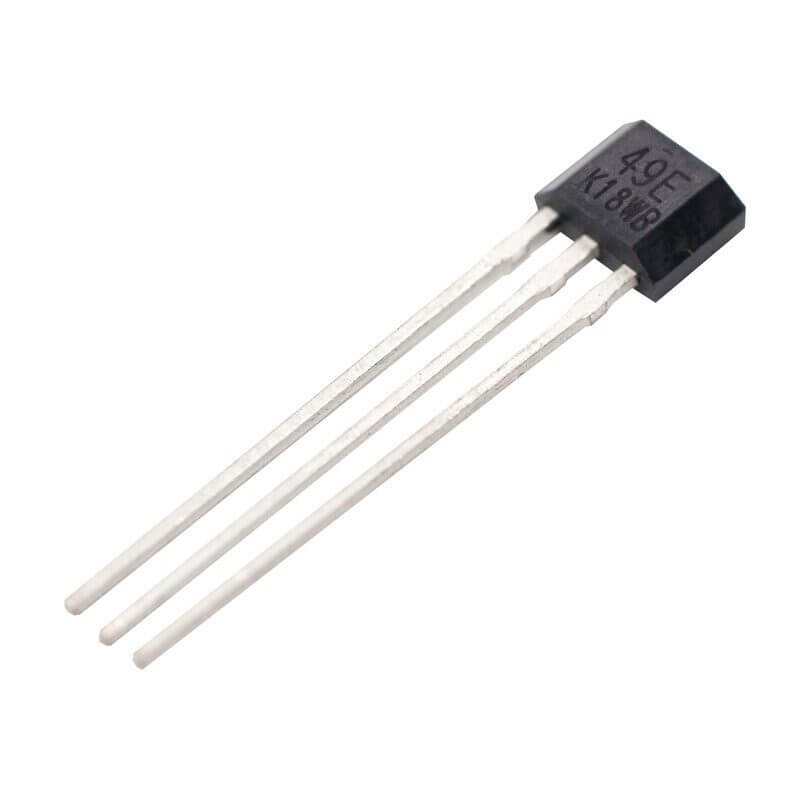
\includegraphics[width=0.25\textwidth]{Hall.jpg}%
					\label{fig:Hall}
					\cite{EfectoHall}
				}
				\hfill
			\end{figure}
			
			\end{enumerate}
			
			\item \textbf{Aceleración}
			
			Los Sensores de aceleración son dispositivos que mide la aceleración experimentada por un objeto en movimiento. Funciona detectando cambios en la velocidad del objeto en una dirección particular. Cuando un objeto acelera, cambia su velocidad en esa dirección, y el sensor de aceleración registra este cambio. \cite{Aceleración} \\
			
			\begin{enumerate}
				\item Todos los sensores de fuerza: De manera parecida a las mediciones de velocidad que se dan a partir de la información de los sensores de posición, pueden encontrarse las aceleraciones como la razón de cambio respecto al tiempo de las velocidades obtenidas por los sensores de velocidad o calculado a partir de las informaciones de posición. Pero ésta no es una manera efi ciente para calcular la aceleración, puesto que impondrá una carga de trabajo pesada sobre la computadora, lo que puede reducir la velocidad de operación del sistema. Otra forma de medir la aceleración es calculando la fuerza que resulta de multiplicar masa por aceleración. \cite{saha2010robotics}\\
			\end{enumerate}
				\begin{figure}[h]Acelerac
				\centering
				\subfloat[Aceleración]{%
					\includegraphics[width=0.25\textwidth]{Aceleración.jpg}%
					\label{fig:Aceleración}
					\cite{ión}
				}
				\hfill
			\end{figure}
			
			\item \textbf{Fuerza}
			
			Una balanza de resorte es un ejemplo de un sensor de
			fuerza en donde se aplica una fuerza, por ejemplo, el peso, al platillo de balanza que causa un desplazamiento, es decir, el resorte se estira. El desplazamiento es entonces una medida de la fuerza. Existen otros tipos de sensores de fuerza, por ejemplo, con base en galgas, utilizando el sensor de efecto Hall, etcétera. \cite{saha2010robotics}\\
			\begin{enumerate}
				\item Galgas extensométricas:
				
				\item Interruptores de límite:
				
				\item Interruptores piezoeléctricos:
				
			\end{enumerate}
		\end{enumerate}
		
	\subsection{Sensores Externos}
	 \begin{enumerate}
		\item \textbf{Tipo de contacto}
		\begin{enumerate}
			\item Interruptores de límite
			\item Interruptores neumáticos
			\item Sensores piezoeléctricos
			\item Transductores de presión
		\end{enumerate}
		\item \textbf{Tipo sin contacto}
		\begin{enumerate}
			\item Sensores de proximidad:  Es un dispositivo que detecta la presencia o ausencia de un objeto dentro de un rango específico sin necesidad de contacto físico. Este tipo de sensor es ampliamente utilizado en aplicaciones industriales y de automatización debido a su capacidad para operar en entornos donde el contacto directo podría ser problemático o dañino.\cite{Prox}\\ 
			\begin{figure}[h]
				\centering
				\subfloat[Sensor de proximidad]{%
					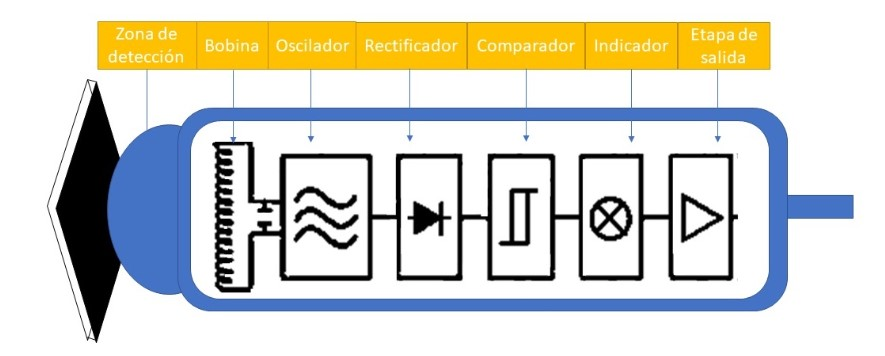
\includegraphics[width=0.20\textwidth]{Prox.jpg}%
					\label{fig:Sensor de proximidad}
					\cite{Prox}
				}
				\hfill
			\end{figure}
			\item Sensores de efecto Hall: Es un dispositivo que utiliza el efecto Hall para detectar campos magnéticos y convertir esta medición en una señal eléctrica. Este tipo de sensor es particularmente útil en aplicaciones donde se requiere la detección de la proximidad o la posición de objetos magnéticos sin necesidad de contacto físico.\cite{EHall}\\ 
			\begin{figure}[h]
				\centering
				\subfloat[Sensor de efecto Hall]{%
					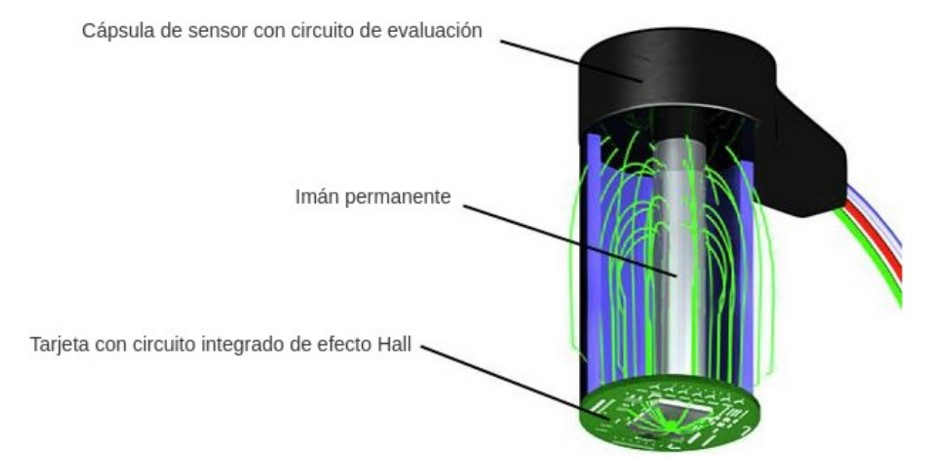
\includegraphics[width=0.20\textwidth]{SHall.jpg}%
					\label{fig:Sensor de efecto Hall}
					\cite{EHall}
				}
				\hfill
			\end{figure}
			\item Sensores de microondas: son dispositivos electrónicos que utilizan radiación de microondas para detectar movimiento, presencia o distancia sin necesidad de contacto físico. Estos sensores son especialmente útiles en aplicaciones donde la detección sin contacto es crucial, como en sistemas de seguridad, automatización industrial y control de tráfico.\cite{microo}\\ 
			\begin{figure}[h]
				\centering
				\subfloat[Sensores de microondas]{%
					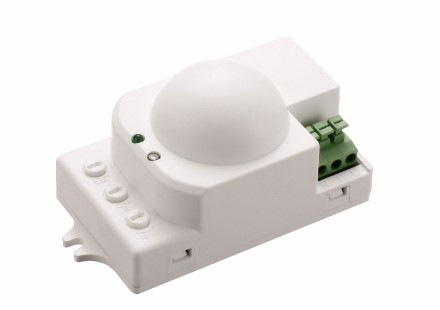
\includegraphics[width=0.20\textwidth]{Microoondas.jpg}%
					\label{fig:Sensores de microondas}
					\cite{microo}
				}
				\hfill
			\end{figure}
			\item Sensores ultrasónicos: Son dispositivos que utilizan ondas sonoras de alta frecuencia para medir distancias y detectar objetos sin contacto físico. Estos sensores son particularmente útiles en aplicaciones industriales y automatización, donde la precisión y la fiabilidad son esenciales.\cite{ultrason}\\ 
			\begin{figure}[h]
				\centering
				\subfloat[Sensores ultrasónicos]{%
					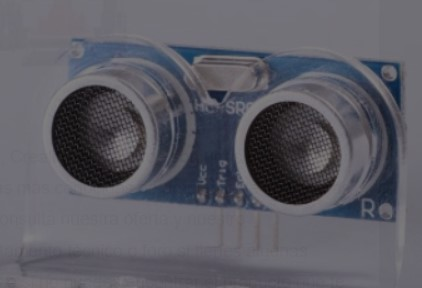
\includegraphics[width=0.20\textwidth]{Ultrasonico.jpg}%
					\label{fig:Sensores ultrasónicos}
					\cite{ultrason}
				}
				\hfill
			\end{figure}
			\item Sensores láser: Son dispositivos ópticos que utilizan un haz de luz láser para medir distancias, posiciones y detectar objetos sin contacto físico. Su capacidad para operar sin necesidad de tocar el objeto a medir los convierte en herramientas valiosas en diversas aplicaciones industriales y tecnológicas.\cite{Slaser}\\ 
			\begin{figure}[h]
				\centering
				\subfloat[Sensores láser]{%
					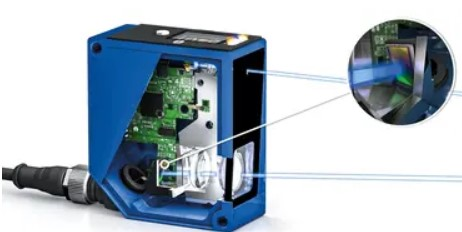
\includegraphics[width=0.15\textwidth]{SensorLaser.jpg}%
					\label{fig:Sensores láser}
					\cite{Slaser}
				}
				\hfill
			\end{figure}
			\item Sensores de visión: Son dispositivos que utilizan tecnología de imagen para detectar y analizar objetos sin necesidad de contacto físico. Estos sensores son parte integral de los sistemas de visión artificial y se emplean en diversas aplicaciones industriales, como inspección de calidad, control de procesos y automatización.\cite{Svision}\\ 
			\begin{figure}[h]
				\centering
				\subfloat[Sensores de visión]{%
					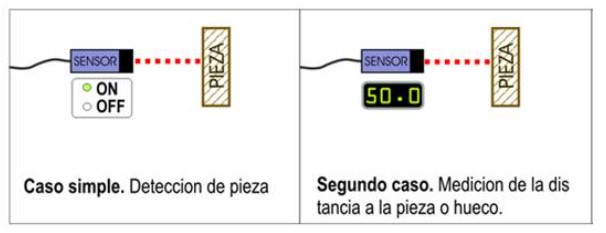
\includegraphics[width=0.20\textwidth]{SensorVision.jpg}%
					\label{fig:Sensores de visión}
					\cite{Svision}
				}
				\hfill
			\end{figure}
		\end{enumerate}
	\end{enumerate}

Para usar dos imágenes como en \autoref{fig:mascotas}, se utilizó \texttt{subfloat}.
% Dos imágenes de mascotas
\begin{figure}[h]
	\centering
	\subfloat[Perro]{%
		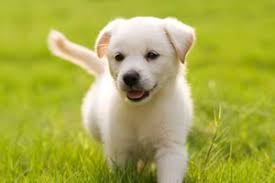
\includegraphics[width=0.4\textwidth]{perro.jpg}%
		\label{fig:perro}
	}
	\hfill
	\subfloat[Gato]{%
		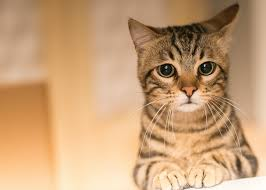
\includegraphics[width=0.4\textwidth]{gato.jpg}%
		\label{fig:gato}
	}
	\caption{Imagen de dos mascotas}
	\label{fig:mascotas}
\end{figure}